\documentclass{zzblmod}
\usepackage{metalogo}
\team{0}	% 组号
\membera{组员A}
\joba{编程}
\memberb{组员B}
\jobb{建模}
\memberc{组员C}
\jobc{建模}

\title{2020B 穿越沙漠}
\tihao{0} % 题号

\begin{document}

\maketitle

\begin{abstract}
	“穿越沙漠”是怎么回事呢,小编也是十分好奇呢
	\keywords{
		最优化模型 \quad
		动态规划 \quad
		静态博弈 \quad
	}
\end{abstract}

\tableofcontents
\newpage

\section{问题重述}

创意平板折叠桌注重于表达木制品的优雅和设计师所想要强调的自动化与功能性。为了增大有效使用面积。设计师以长方形木板的宽为直径截取了一个圆形作为桌面,又将木板剩余的面积切割成了若干个长短不一的木条,每根木条的长度为平板宽到圆上一点的距离,分别用两根钢筋贯穿两侧的木条,使用者只需提起木板的两侧,便可以在重力的作用下达到自动升起的效果,相互对称的木条宛如下垂的桌布,精密的制作工艺配以质朴的木材,让这件工艺品看起来就像是工业革命时期的机器。

\subsection{问题的提出}

围绕创意平板折叠桌的动态变化过程、设计加工参数,本文依次提出如下问题:

(1)给定长方形平板尺寸 ($120 cm \times 50 cm \times 3 cm$),每根木条宽度(2.5 cm),连接桌腿木条的钢筋的位置,折叠后桌子的高度(53 cm)。要求建立模型描述此折叠桌的动态变化过程,并在此基础上给出此折叠桌的设计加工参数和桌脚边缘线的数学描述。

(2)......


\section{模型的假设}

\begin{itemize}
	\item 忽略实际加工误差对设计的影响;
	\item 木条与圆桌面之间的交接处缝隙较小,可忽略;
	\item 钢筋强度足够大,不弯曲;
	\item 假设地面平整。
\end{itemize}

\section{符号说明}
\begin{center}
	\begin{tabular}{cc}
		\hline
		\makebox[0.3\textwidth][c]{符号}	&  \makebox[0.4\textwidth][c]{意义} \\ \hline
		D	    & 木条宽度(cm) \\ \hline
		L	    & 木板长度(cm)  \\ \hline
	\end{tabular}
\end{center}

\section{问题分析}

\subsection{问题一分析}
题目要求建立模型描述折叠桌的动态变化图,由于在折叠时用力大小的不同,我们不能描述在某一时刻折叠桌的具体形态,但我们可以用每根木条的角度变化来描述折叠桌的动态变化。插入参考文献\cite{bib:one}。

问题流程图:
\begin{figure}[!h]
	\centering
	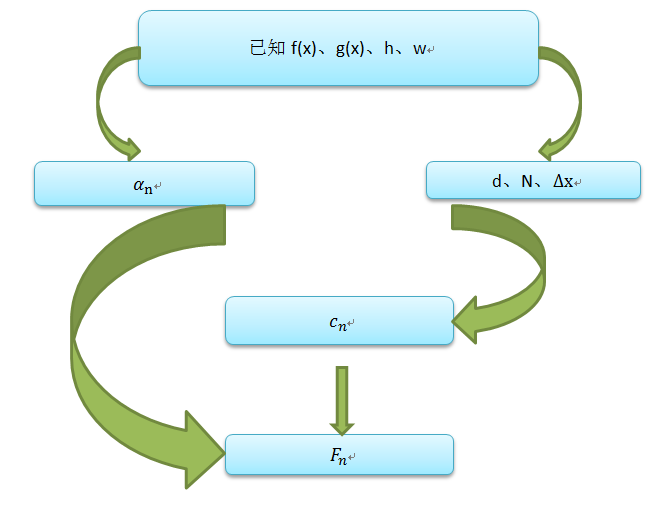
\includegraphics[width=.6\textwidth]{1.png}
	\caption{问题三流程图}
\end{figure}

\section{绘制普通三线表格}
表格应具有三线表格式,因此常用 booktabs宏包,其标准格式如表~\ref{tab001}~所示。
\begin{table}[!htbp]
	\caption{标准三线表格}\label{tab001} \centering
	\begin{tabular}{ccccc}
		\toprule[1.5pt]
		$D$(in) & $P_u$(lbs) & $u_u$(in) & $\beta$ & $G_f$(psi.in)\\
		\midrule[1pt]
		5 & 269.8 & 0.000674 & 1.79 & 0.04089\\
		10 & 421.0 & 0.001035 & 3.59 & 0.04089\\
		20 & 640.2 & 0.001565 & 7.18 & 0.04089\\
		\bottomrule[1.5pt]
	\end{tabular}
\end{table}

%参考文献
\begin{thebibliography}{9}%宽度9
	\bibitem{bib:one} GAO L, GONDA I, SUN H, et al. The Tomato Pan-Genome Uncovers New Genes and a	Rare Allele Regulating Fruit Flavor[J]. Nature Genetics, 2019:1.
	\bibitem{bib:two} ....
\end{thebibliography}

\appendix %%附录
\section{代码}
\subsection{第一问不挖矿--matlab 源程序}
\begin{lstlisting}[language=matlab]
p = [
0 1 0 0 0 0 0 0 0 0 0 0 0 0 0 0 0 0 0 0 0 0 0 0 1 0 0
0 0 1 1 0 0 0 0 0 0 0 0 0 0 0 0 0 0 0 0 0 0 0 0 0 0 0
0 1 0 1 0 0 0 0 0 0 0 0 0 0 0 0 0 0 0 0 0 0 0 0 1 0 0
0 0 1 0 1 0 0 0 0 0 0 0 0 0 0 0 0 0 0 0 0 0 0 1 1 0 0
0 0 0 1 0 1 0 0 0 0 0 0 0 0 0 0 0 0 0 0 0 0 0 1 0 0 0
0 0 0 0 1 0 1 0 0 0 0 0 0 0 0 0 0 0 0 0 0 0 1 1 0 0 0
0 0 0 0 0 1 0 1 0 0 0 0 0 0 0 0 0 0 0 0 0 1 0 0 0 0 0
0 0 0 0 0 0 1 0 1 0 0 0 0 0 0 0 0 0 0 0 0 1 0 0 0 0 0
0 0 0 0 0 0 0 1 0 1 0 0 0 0 1 1 1 0 0 0 0 1 0 0 0 0 0
0 0 0 0 0 0 0 0 1 0 1 0 1 0 0 0 0 0 0 0 0 0 0 0 0 0 0
0 0 0 0 0 0 0 0 0 1 0 1 1 0 0 0 0 0 0 0 0 0 0 0 0 0 0
0 0 0 0 0 0 0 0 0 0 1 0 1 1 0 0 0 0 0 0 0 0 0 0 0 0 0
0 0 0 0 0 0 0 0 0 1 1 1 0 1 1 0 0 0 0 0 0 0 0 0 0 0 0
0 0 0 0 0 0 0 0 0 0 0 1 1 0 1 1 0 0 0 0 0 0 0 0 0 0 0
0 0 0 0 0 0 0 0 1 1 0 0 1 1 0 1 0 0 0 0 0 0 0 0 0 0 0
0 0 0 0 0 0 0 0 0 0 0 0 0 1 1 0 1 1 0 0 0 0 0 0 0 0 0
0 0 0 0 0 0 0 0 1 0 0 0 0 0 0 1 0 1 0 0 1 0 0 0 0 0 0
0 0 0 0 0 0 0 0 0 0 0 0 0 0 0 1 1 0 1 1 0 0 0 0 0 0 0
0 0 0 0 0 0 0 0 0 0 0 0 0 0 0 0 0 1 0 1 0 0 0 0 0 0 0
0 0 0 0 0 0 0 0 0 0 0 0 0 0 0 0 0 1 1 0 1 0 0 0 0 0 0
0 0 0 0 0 0 0 0 1 0 0 0 0 0 0 0 1 0 0 1 0 1 1 0 0 0 1
0 0 0 0 0 0 1 1 1 0 0 0 0 0 0 0 0 0 0 0 1 0 1 0 0 0 0
0 0 0 0 0 1 0 0 0 0 0 0 0 0 0 0 0 0 0 0 1 1 0 1 0 1 0
0 0 0 1 1 1 0 0 0 0 0 0 0 0 0 0 0 0 0 0 0 0 1 0 1 1 0
1 0 1 1 0 0 0 0 0 0 0 0 0 0 0 0 0 0 0 0 0 0 0 1 0 1 0
0 0 0 0 0 0 0 0 0 0 0 0 0 0 0 0 0 0 0 0 0 0 1 1 1 0 1
0 0 0 0 0 0 0 0 0 0 0 0 0 0 0 0 0 0 0 0 1 0 0 0 0 1 0
];
inf = 99999999;
n = size(p,1);

dis = p;
for i = 1:27
    for j = 1:27
        if dis(i,j)==0
            dis(i,j) = inf;
        end
    end
end

% use Floyd to calculate
for k = 1:n
    for i=1:n
        for j=1:n
            if dis(i,k)+dis(k,j)<dis(i,j)
                dis(i,j) = dis(i,k) + dis(k,j);
            end
        end
    end
end

dis = dis.*(ones(27) - diag(ones(1, 27)));

weather = [2, 2, 1, 3, 1, 2, 3, 1, 2, 2, 3, 2, 1, 2, 2, 2, 3, 3, 2, 2, 1, 1, 2, 1, 3, 2, 1, 1, 2, 2];
w_cost = [5 8 10];
f_cost = [7 6 10];
weight_limit = 1000;
day_limit = 30;
price_w = 5;
price_f = 10;
weight_w = 3;
weight_f= 2;

sumw = 0;
sumf = 0;
dest = 27;

i=0;
day=0;

while day<dis(1, dest)
    i=i+1;
    if weather(i)~=3
        day=day+1;
        sumw = sumw + 2 * w_cost(weather(i));
        sumf = sumf + 2 * f_cost(weather(i));
    else
        sumw = sumw + w_cost(weather(i));
        sumf = sumf + f_cost(weather(i));
    end
end

left = 10000 - sumw*price_w - sumf*price_f;
left
sumw
sumf

\end{lstlisting}

\end{document}